\documentclass[preprint,12pt, a4paper]{elsarticle}

\usepackage{amssymb}
\usepackage{lineno}
\usepackage{float}
\usepackage{hyperref}
\usepackage{listings}
\lstset{language=Python}

\restylefloat{table}

\journal{SoftwareX}

\begin{document}

\begin{frontmatter}

\title{geometric-smote: A package for flexible and efficient over-sampling}

\author{Georgios Douzas}
\ead{gdouzas@novaims.unl.pt}

\author{Fernando Bacao\corref{nova}}
\ead{bacao@novaims.unl.pt}

\address{NOVA Information Management School, Universidade Nova de Lisboa}

\cortext[nova]{Postal Address: NOVA Information Management School, Campus de Campolide, 1070-312 Lisboa, Portugal, Telephone: +351 21 382 8610}

\begin{abstract}
Classification of imbalanced datasets is a challenging task for standard algorithms. G-SMOTE is a state-of-the-art oversampling algorithm that has been shown to outperform the popular SMOTE oversampler and its variations. In this paper, a Python implementation of G-SMOTE is provided that integrates with the Scikit-Learn ecosystem. Therefore, machine learning researchers and practitioners can benefit from its use in a straightforward manner.
\end{abstract}

\begin{keyword}
Machine learning \sep Imbalanced learning problem \sep Oversampling
\end{keyword}

\end{frontmatter}

\begin{table}[H]
\begin{tabular}{|p{6.5cm}|p{6.5cm}|}
\hline
Code metadata & \\
\hline
Current code version & v0.1.2 \\
\hline
Permanent link to code/repository used for this code version & \url{https://github.com/AlgoWit/geometric-smote} \\
\hline
Legal Code License & MIT \\
\hline
Code versioning system used & git \\
\hline
Software code languages, tools, and services used & Python, Travis CI, AppVeyor, Read the Docs, Codecov, CircleCI, zenodo, Anaconda Cloud \\
\hline
Compilation requirements, operating environments \& dependencies & Linux, Mac OS, Windows \\
\hline
If available Link to developer documentation/manual & \url{https://geometric-smote.readthedocs.io/} \\
\hline
Support email for questions & \href{mailto:georgios.douzas@gmail.com}{georgios.douzas@gmail.com} \\
\hline
\end{tabular}
\caption{Code metadata}
\label{} 
\end{table}

\linenumbers

%% main text

\section{Motivation and significance}
\label{motivation}

\subsection{Introduction}
\label{introduction}

The imbalanced learning problem is defined as a machine learning classification task using datasets with binary or multi-class targets where one of the classes, called the majority class, outnumbers significantly the remaining classes, called the minority class(es) \cite{Chawla2003}. Learning from imbalanced data is a frequent non-trivial problem for academic researchers and industry practitioners. The imbalance learning problem can be found in multiple domains such as chemical and biochemical engineering, financial management, information
technology, security, business, agriculture or emergency management \cite{Haixiang2017}.

The Imbalance Ratio (IR) is defined as the ratio between the number of samples of the majority class and each of the minority classes. IR values between 100 and 100.000 have been observed \cite{Chawla2002}, \cite{Barua2014}. Standard machine learning classification algorithms induce a bias towards the majority class during training. This results in low performance when metrics suitable for imbalanced data are used for the classifier's evaluation. Figure \ref{fig:imbalanced} shows an example of imbalanced data in two dimensions and the resulting decision boundary of a typical classifier when they are used as a training set.

\begin{figure}[H]
	\centering
    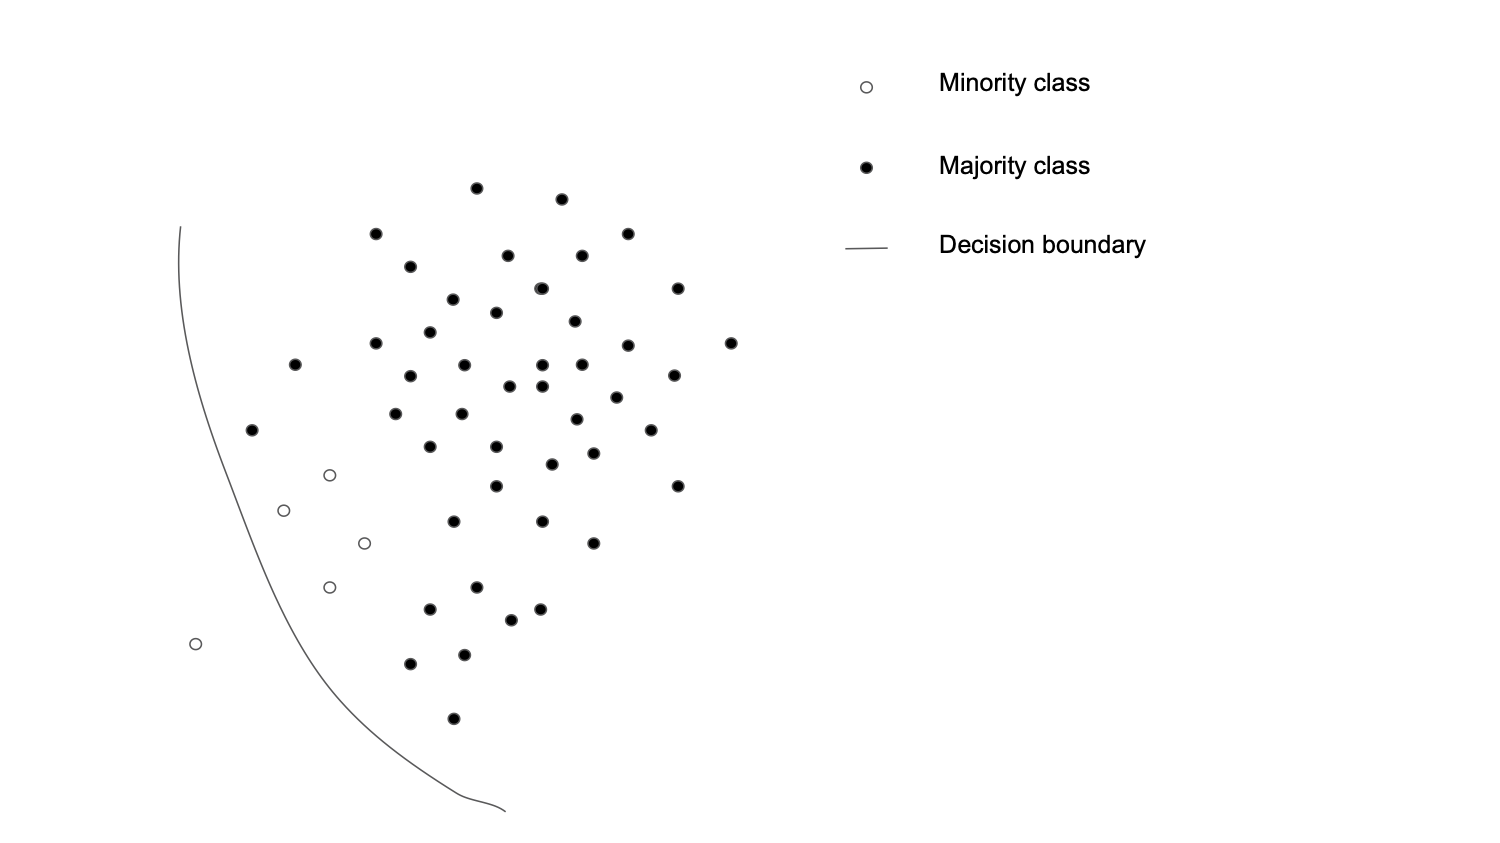
\includegraphics[width=14cm, keepaspectratio]{../analysis/imbalanced_problem}
    \caption{Imbalanced data in two dimensions. The decision boundary of a classifier shows a bias towards the majority class,}
    \label{fig:imbalanced}
\end{figure}

\subsection{Oversampling algorithms}
\label{oversampling}

Various approaches have been proposed to deal with the imbalanced learning problem \cite{Fernandez2013}. One general approach is the modification at the data level by oversampling the minority class(es). Synthetic Minority
Oversampling Technique (SMOTE) \cite{Chawla2002} is the most popular oversampling algorithm. It generates synthetic instances along a line segment that joins minority class instances. Although SMOTE has been shown to be effective for oversampling imbalanced data, it also has some weaknesses \cite{He2009}. In order to improve the quality of the generated data, many variations of SMOTE have been proposed. Nevertheless, all of these variations use the same data generation mechanism, i.e. linear interpolation between minority class samples.

A Python implementation of SMOTE and a couple of its variations is available in the \href{https://imbalanced-learn.org/stable/}{Imbalanced-Learn} \cite{Lemaitre2016} library. Imbalanced-Learn is fully compatible with \href{https://scikit-learn.org/stable/}{Scikit-Learn} \cite{Pedregosa2011}, one of the most popular machine learning libraries. 

\subsection{Geometric SMOTE}
\label{gsmote}

Geometric SMOTE (G-SMOTE) \cite{Douzas2019} uses a different approach compared to existing SMOTE's variations. More specifically, G-SMOTE oversampling algorithm substitutes the data generation mechanism of SMOTE by defining a flexible geometric region around each minority class instance and generating synthetic instances inside the boundaries of this region. The algorithm requires the selection of the hyperparameters \texttt{truncation\_factor}, \texttt{deformation\_factor}, \texttt{selection\_strategy} and \texttt{k\_neighbors}. The first three of them, called geometric hyperparameters, control the shape of the geometric region while the later adjusts its size. Figure \ref{fig:smote_vs_gsmote} presents a visual comparison between the data generation mechanisms of SMOTE and G-SMOTE.

\begin{figure}[H]
	\centering
	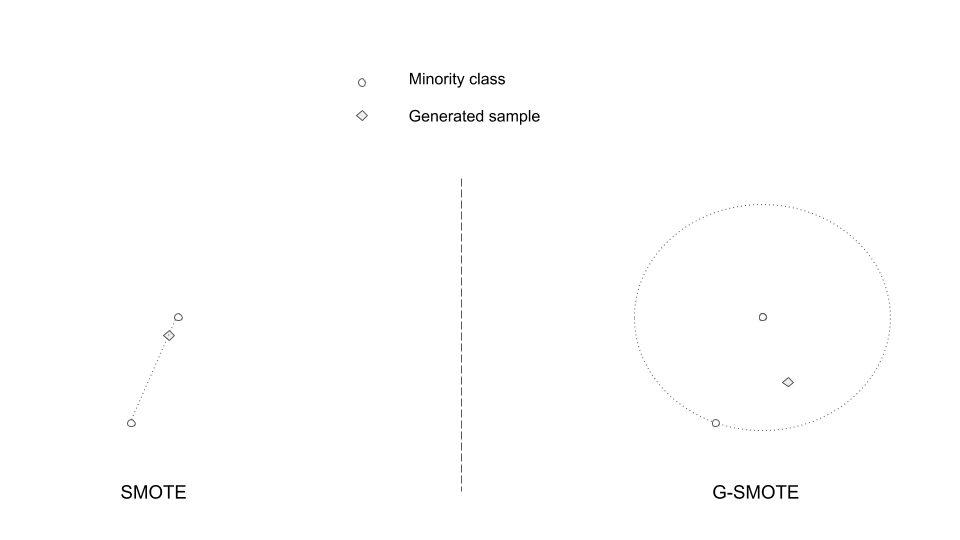
\includegraphics[width=1\linewidth]{../analysis/smote_vs_gsmote}
	\caption{Comparison between the data generation mechanisms of SMOTE and G-SMOTE. SMOTE uses linear interpolation, while G-SMOTE defines a circle as the permissible data generation area.}
	\label{fig:smote_vs_gsmote}
\end{figure}

G-SMOTE algorithm has been shown to outperform SMOTE across 69 imbalanced datasets for various classifiers and evaluation metrics. This paper, presents a Python implementation of G-SMOTE. In section 2, the software description is given while section 3 provides a demonstrative example of its functionalities.

\section{Software description}

The \texttt{geometric-smote} project is written in Python 3.7. It contains an object-oriented implementation of the G-SMOTE algorithm as well as an extensive \href{https://geometric-smote.readthedocs.io/}{online documentation}. The implementation provides an API that is compatible with Imbalanced-Learn and Scikit-Learn libraries, therefore it makes full use of various features that support standard machine learning functionalities.

\subsection{Software Architecture}
\label{architecture}

The \texttt{geometric-smote} project contains the Python package \texttt{gsmote}. The main module of \texttt{gsmote} is called \texttt{geometric-smote}. It contains the class \texttt{GeometricSMOTE} that implements the G-SMOTE algorithm. The initialization of an \texttt{GeometricSMOTE} instance includes G-SMOTE's hyperparameters that control the generation of synthetic data. Additionally, \texttt{GeometricSMOTE} inherits from the \texttt{BaseOverSampler} class of Imbalanced-Learn library. Therefore, an instance of \texttt{GeometricSMOTE} class provides the \texttt{fit} and \texttt{fit\_resample} methods, the two main methods for resampling as explained in subsection \ref{functionality}. This is achieved by implementing the \texttt{\_fit\_resample} abstract method of the parent class \texttt{BaseOverSampler}. More specifically, the function \texttt{\_make\_geometric\_sample} implements the data generation mechanism of G-SMOTE as shortly described in section \ref{gsmote}. This function is called in the \texttt{\_make\_geometric\_samples} method of the \texttt{GeometricSMOTE} class in order to generate the appropriate number of synthetic data for a particular minority class. Finally, the method \texttt{\_make\_geometric\_samples} is called in \texttt{\_fit\_resample} method to generate synthetic data for all minority classes. Figure \ref{fig:class_diagram} provides a visual representation of the above classes and functions hierarchy.

\begin{figure}[H]
	\centering
	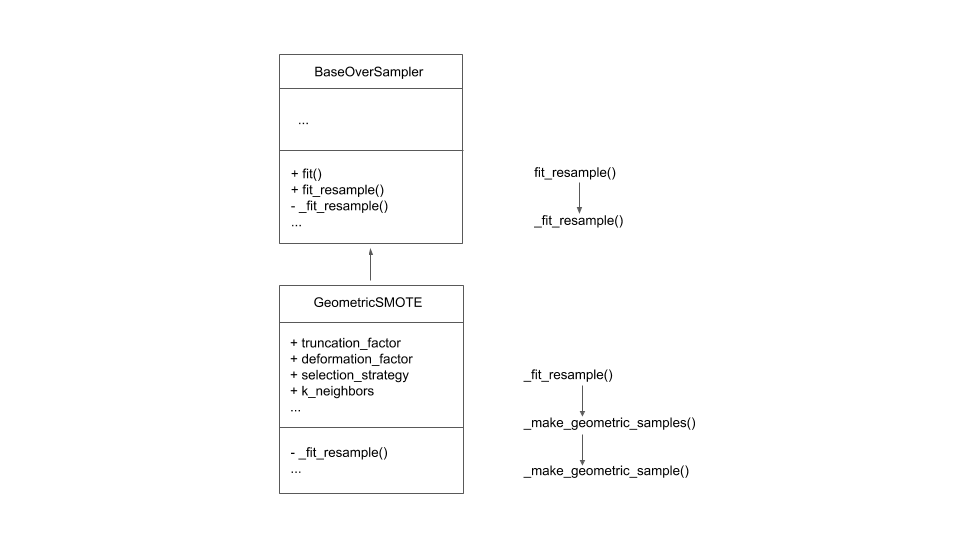
\includegraphics[width=1\linewidth]{../analysis/class_diagram}
	\caption{UML class diagrams and callgraphs of main classes and methods.}
	\label{fig:class_diagram}
\end{figure}

\subsection{Software Functionalities}
\label{functionality}

As it was mentioned in subsection \ref{architecture}, the class \texttt{GeometricSMOTE} represents the G-SMOTE oversampler. The intializer of \texttt{GeometricSMOTE} includes the following G-SMOTE's hyperparameters: \texttt{truncation\_factor}, \texttt{deformation\_factor}, \texttt{selection\_strategy} and \texttt{k\_neighbors} as explained in subsection \ref{gsmote}. Once the \texttt{GeometricSMOTE} object is initialized with a specific parametrization, it can be used to resample the imbalanced data represented by the input matrix \texttt{X} and the target labels \texttt{y}. Following the Scikit-Learn API, both \texttt{X}, \texttt{y} are array-like objects of appropriate shape.

Resampling is achieved by using the two main methods of \texttt{fit} and \texttt{fit\_resample} the \texttt{GeometricSMOTE} object. More specifically, both of them take as input parameters the \texttt{X} and \texttt{y}. The first method computes various statistics which are used to resample \texttt{X} while the second method does the same but additionally returns a resampled version of \texttt{X} and \texttt{y}.

The \texttt{geometric-smote} project has been designed to integrate with the Imbalanced-Learn toolbox and Scikit-Learn ecosystem. Therefore the \texttt{GeometricSMOTE} object can be used in a machine learning pipeline, through Imbalanced-Learn's class \texttt{Pipeline}, that automatically combines \texttt{samplers}, \texttt{transformers} and \texttt{estimators}. The next section provides examples of the above functionalities.

\section{Illustrative Examples}

\subsection{Basic example}

An example of resampling multi-class imbalanced data using the \texttt{fit\_resample} method is presented in Listing \ref{lst:basic}. Initially, 
a 3-class imbalanced dataset is generated. Next, \texttt{GeometricSMOTE} object is initialized with default values for the hyperparameters, i.e. $\texttt{truncation\_factor} = 1.0$, $\texttt{deformation\_factor}=0.0$, $\texttt{selection\_strategy}=\textrm{combined}$. Finally, the object's \texttt{fit\_resample} method is used to resample the data. Printing the class distribution before and after resampling confirms that the resampled data are perfectly balanced. The resampled data \texttt{X\_res}, \texttt{y\_res} can be used as training data for any classifier in the place of \texttt{X}, \texttt{y}.

\begin{lstlisting}[caption={Resampling of imbalanced data using the \texttt{fit\_resample} method.},label={lst:basic}]
# Import classes and functions.
from collections import Counter
from gsmote import GeometricSMOTE
from sklearn.datasets import make_classification

# Generate an imbalanced 3-class dataset.
X, y = make_classification(
    random_state=23, 
    n_classes=3, 
    n_informative=5,
    n_samples=500,
    weights=[0.8, 0.15, 0.05]
)

# Create a GeometricSMOTE object with default hyperparameters.
gsmote = GeometricSMOTE(random_state=10)

# Resample the imbalanced dataset.
X_res, y_res = gsmote.fit_resample(X, y) 

# Print number of samples per class for initial and resampled data. 
init_count = list(Counter(y).values())
resampled_count = list(Counter(y_res).values())

print(f'Initial class distribution: {init_count}.') 
# Initial class distribution: [400, 75, 25].

print(f'Resampled class distribution: {resampled_count}.')
# Resampled class distribution: [400, 400, 400].
\end{lstlisting}

\subsection{Machine learning pipeline}

The \texttt{GeometricSMOTE} object can be used as a part of a machine learning pipeline. Listing \ref{lst:pipeline} presents a pipeline composed by a G-SMOTE oversampler, a PCA tranformation and a decision tree classifier. The pipeline is trained on imbalanced binary-class data and evaluated on a hold-out set. The user applies the process in a small number of steps while the internal details of the calculations are hidden.

\begin{lstlisting}[caption={Training and evaluation of a machine learning pipeline that contains the \texttt{GeometricSMOTE} object.},label={lst:pipeline}]
# Import classes and functions.
from gsmote import GeometricSMOTE
from sklearn.datasets import make_classification
from sklearn.decomposition import PCA
from sklearn.tree import DecisionTreeClassifier
from sklearn.model_selection import train_test_split
from sklearn.metrics import f1_score
from imblearn.pipeline import make_pipeline

# Generate an imbalanced binary-class dataset.
X, y = make_classification(
	random_state=23, 
	n_classes=2, 
	n_samples=500,
	weights=[0.8, 0.2]
)

# Split the data to training and hold-out sets.
X_train, X_test, y_train, y_test = train_test_split(X, y, random_state=0)

# Create the pipeline's objects with default hyperparameters.
gsmote = GeometricSMOTE(random_state=11)
pca = PCA()
clf = DecisionTreeClassifier(random_state=3)

# Create the pipeline.
pip = make_pipeline(gsmote, pca, clf)

# Fit the pipeline to the training set.
pip.fit(X_train, y_train)

# Evaluate the pipeline on the hold-out set using the F-score.
test_score = f1_score(y_test, pip.predict(X_test))

print(f'F-score on hold-out set: {test_score}.')
# F-score on hold-out set: 0.7.
\end{lstlisting}

\section{Impact and conclusions}

Classification of imbalanced datasets is a challenging task for standard machine learning algorithms. G-SMOTE, as a enhancement of the SMOTE data generation mechanism, provides a flexible and effective way for resampling the imbalanced data that has been shown to outperform SMOTE and its variations. Machine learning researchers and industry practitioners can benefit from using G-SMOTE in their work since the imbalanced learning problem is an active research area as well as a common feature of real-world applications.

The \texttt{geometric-smote} project provides a Python implementation of the state-of-the-art oversampling algorithm G-SMOTE. The main advantage of this implementation is that it is built on top of Scikit-Learn's ecosystem. Therefore, using the oversampler in typical machine learning workflows is an effortless task. Also, the public API of the main class \texttt{GeometricSMOTE} is identical to the one implemented in Imbalanced-Learn for all oversamplers. Consequently, users of Imbalanced-Learn and Scikit-Learn, that apply oversampling on imbalanced data, can integrate the \texttt{gsmote} package in their existing work in a straightforward manner.

\section{Conflict of Interest}

We wish to confirm that there are no known conflicts of interest associated with this publication and there has been no significant financial support for this work that could have influenced its outcome.

\bibliography{references}
\bibliographystyle{elsarticle-num}
\end{document}
\endinput

